\chapter{Approach}
\label{ch:approach}
In the following section, we introduce our proposed security approach for substation automation systems.
With the aim of securing the time-critical communication between resource-constrained devices in a time-variable environment, we propose a security framework for \textbf{S}erver-aided \textbf{A}BAC with \textbf{Z}ero-RTT \textbf{E}ncryption (SAZE).
The SAZE ("Sassy") security framework is able to prevent and mitigate cyberattacks by providing security mechanisms and enforcing mandatory communication policies.

The introduction and discussion of the proposed approach is organized as follows.
At the beginning of this chapter in \autoref{sec:approach:system_model}, we discuss the field of application of the proposed approach by introducing a system model and defining its requirements.
Based on the presented system model and requirements, we introduce the security model and architecture of the SAZE security framework in \autoref{sec:approach:security_model}.
The two main SAZE concepts server-aided ABAC and zero-RTT encryption are introduced in \autoref{sec:approach:sa} and \autoref{sec:approach:ze}.
In \autoref{sec:approach:realization} we present the planned realization of the SAZE security framework.
Subsequently, we present the proposed evaluation strategies and metrics of the security framework in \autoref{sec:approach:evaluation}.
Finally, in \autoref{sec:approach:limitations} we discuss limitations of the proposed approach.
%\todo{Own idea, concept, protocol, evaluation, proof, testing, expected benefits and limitations}
%\todo{SECURITY: Security Goals (CIA + Privacy Preserving)}
%\todo{IDEA: Wrap packages of arbitrary protocols by encripting payload of ethernet package, and adding a new header with ABAC-SS information. Maybe as HW Middleware? If other endpoint does not support the ABAC-SS wrapping fall back to proofing endpoint via identity provider only.}
%\todo{PERF EVALUATION: 1. Run approach on network simulator, and 2. Run approach on raspberry pi's representing different roles like server, DER, user \dots}

\section{System Model}
\label{sec:approach:system_model}
In the following sections, we introduce the system model of the SAZE approach.
The system model serves the purpose of delimiting the scope and area of application of the proposed approach.

The area of application of the proposed approach is the power system domain.
More specifically, the proposed approach is tailored to the communication and control systems of substations in the electricity grid.
The communication and control equipment of an ICS is referred to as secondary equipment.
The entirety of secondary equipment of a substation is referred to as Substation Automation System (SAS) \cite{Padilla2015}.
Although the proposed approach is tailored to the power system domain and substation environment, its main concepts may also be applied to other ICS with similar requirements and constraints.

\subsection{Architecture}
The architecture of the presented system model and SAS respectively is based on the IEC 61850 standard \cite{IEC61850P5}.
The presented system model architecture consists of four layers called network level, station level, bay level, and process level.
The process, bay, and station level represent the internal layers of a SAS architecture.
The SAS architecture containing the process, bay, and station level as well as the station and process bus further discussed in \autoref{sec:approach:system_model:communication} is shown in \autoref{fig:substation_architecture}.
The network level represents a SAS-external layer to integrate multiple SAS instances into a comprehensive power system.
Each of the four layers consists of different devices and provides different control and automation functions:
\begin{enumerate}
    \item Process Level: The process level provides functions to interact with the physical process via sensors and actuators.
    As a consequence, SAS devices located at the process level provide interfaces to the physical process.
    In other words, devices located at the process level transform analog measurement signals or control signals into digital values and vice versa.
    Devices restricted to the transformation and provision of measurement and control values are referred to as Merging Units (MU).
    Moreover, IEDs can be employed to combine MU functions with higher-level functions such as protection or communication tasks.

    \item Bay Level: The bay level provides common functions of so-called bays of a SAS.
    As stated by the \citeauthor{IEC61850P5} \cite{IEC61850P5}, a bay represents a closely connected subpart of a substation with common functionality.
    The devices at bay level supervise the operation of lower-level devices of a SAS bay.
    Consequently, a supervising bay level device is referred to as bay controller or bay protection.

    \item Station Level: The station level provides functions related to the substation as a whole.
    Therefore, the station level comprises devices required for on-site and remote monitoring and control of the substation.
    Devices at the station level include Human Machine Interfaces (HMI) for substation operators as well as Wide Area Network (WAN) gateways like SCADA RTUs.

    \item Network Level: The network level provides higher-level functions exceeding the scope of a single SAS.
    The network level devices include supervisory monitoring and control devices like SCADA MTUs.
\end{enumerate}
\begin{figure}
	\centering
	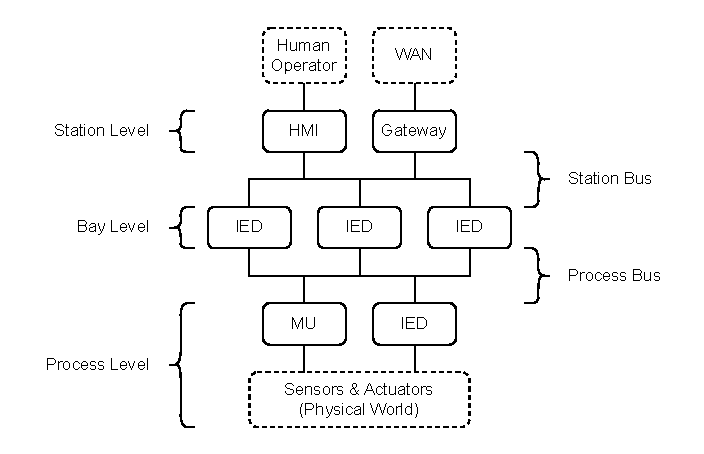
\includegraphics[width=1.0\linewidth]{figures/substation_architecture.drawio.pdf}
	\caption{The internal SAS architecture consisting of devices located on three layers called system level, bay level, and process level connected via station bus and process bus.}
	\label{fig:substation_architecture}
\end{figure}

\subsection{Communication}
\label{sec:approach:system_model:communication}
In the following, we discuss the communication between devices of the presented system model.
For this purpose, we firstly identify different communication characteristics based on which communication relationships and messages can be classified.
Secondly, we define three messages types for time-critical ICS and SAS communication.
Lastly, we discuss the bus-based device interactions occurring in the above-mentioned four layer system model.

\subsubsection{Classification Characteristics}
The communication relationships between devices can be classified using different communication characteristics.
Topological communication characteristics can be used to classify the device relationships based on their relative or absolute location within the system model.
Accordingly, communication can either occur between devices on the same layer or different layers of the system model.
Communication on the same layer of the system model is referred to as horizontal communication, whereas communication between devices on different layers is referred to as vertical communication.
Moreover, communication can occur between devices of the same or different subsystems.
Communication between devices of the same subsystem is classified as (subsystem) internal communication, whereas communication relationships including an external device are classified as (subsystem) external communication.
Furthermore, a communication relationship is not limited to a single receiver (unicast) but rather a group of devices (multicast) or all devices (broadcast) may receive a sender's message.

Besides the topology-based classification, communication relationships can be classified based on their continuity.
Continuous, session-oriented, or stateful communication requires an initial session establishment between the involved devices.
While the first message exchange requires additional initialization overhead, subsequent latencies might benefit from the established communication session.
Discontinuous, message-oriented, or stateless communication enables communication without initial overhead for the involved devices.
Consequently, discontinuous communication does not lead to latency emerging from session initialization and management.

Since communication in ICS and SAS is time-critical, communication relationships can be classified based on their communication latency constraints.
Within the scope of the proposed approach, we define communication latency as sum of processing times and transmission times required to exchange information between involved devices.
The transmission time is the time required to transmit a message over a network link with a specific throughput.
The processing time represents the time required for a device to send, forward, or receive a message or packet.
For intermediate network devices like routers and switches the processing time depends on queuing delay and forwarding delay.
For the sender and receiver of a message or packet the processing time consists of enqueue and dequeue delays, cryptographic overhead, and message coding.
As a consequence, the communication latency represents the time required for a message from being put into the sending buffer at the sender to the point when the message is taken from the receiving buffer at the receiver.

\subsubsection{Message Types}
The defined message types of the presented system model are based on the classification characteristics defined above and on the message types and performance classes of the IEC 61850 standard \cite{IEC61850P5}.
The defined message type as well as their typical communication topology, continuity, and latency constraints are shown in \autoref{tab:message_types}.

The low latency message type corresponds to the IEC 61850 \cite{IEC61850P5} message types 1A and 4.
The low latency messages are used for SAS-internal exchange of sampled values and state values.
In IEC 61850 compliant substations the sampled values are exchanged using the Sampled Values (SV) protocol between MUs and IEDs (vertical) or between MUs (horizontal).
Moreover, state values and state changes are exchanged horizontally between IEDs using the Generic Object Oriented Substation Events (GOOSE) protocol.

The medium latency message type corresponds to the IEC 61850 message types 1B and 2.
The medium latency messages are used for internal and external as well as horizontal and vertical session-based client-server communication.
In IEC 61850 substations IEDs use the Manufacturing Message Specification (MMS) protocol to communicate with other IEDs and higher-level devices.

The high latency message type corresponds to the IEC 61850 message types 3 and 5.
This message type is used for HMI interactions as well as non-time-critical operations like file transfers.
In IEC 61850 substations MMS and SCADA protocols are used for high latency communication.
\begin{table}
    \centering
    \caption{Message types of the presented system model classified with regard to their topology, continuity, and latency constraints of the communication relationships.}
    \label{tab:message_types}
    \begin{tabular}{l c c c c c}
    \toprule
    \multicolumn{1}{c}{Message Type} & \multicolumn{3}{c}{Topology} & Continuity & Latency\\
    & Externality & Verticality & Receiver & & Constraint\\
    \midrule
    Low Latency & Internal & Horiz./Vert. & Multicast & Message-Based & 3 ms\\
    Medium Latency & Int./Ext. & Horiz./Vert. & Unicast & Session-Based & 20-100 ms\\
    High Latency & External & Vert. & Unicast & Session-Based & 500 ms\\
    \bottomrule
    \end{tabular}
    \end{table}

\subsubsection{Communication Buses}
The presented system model uses a bus-based approach for message exchange between the system architecture layers.
The approach as well as the two concrete buses used are based on the IEC 61850 standard \cite{IEC61850P5}.
The first bus is referred to as process bus and is located between the bay level and the process level.
The process bus is used for time-critical message-based publisher-subscriber communication.
Consequently, GOOSE and SV are the IEC 61850 protocols used for process bus communication.

The second bus is referred to as station bus and is located between the station level and the bay level.
The station bus connects IEDs at the bay level with each other as well as with gateways and interfaces at the station level.
The communication at the station bus is typically session-based unicast communication with less strict time requirements compared to the process bus.

%\subsection{Threats}
%\todo{System Threats + Adversaries + Attack Trees}

\subsection{Requirements}
\todo{Requirements: Security, Performance, Interoperability, Safety, Availability -> Link to different Busses/Devices}
\subsubsection{Security}
\subsubsection{Safety}
\subsubsection{Availability}
\subsubsection{Performance}
\subsubsection{Interoperability}

\section{Security Model: Server-Aided ABAC with Zero-RTT Encryption (SAZE)}
\label{sec:approach:security_model}
\subsection{Security Architecture}
\todo{Architecture: SAZE Components \& Layers \& Busses}
\subsubsection{Layers \& Buses}
\subsubsection{Components}
\subsubsection{Stakeholders}

\subsection{Security Policies}
\todo{Security Policies -> Link to Requirements \& Attacks}

\section{Server-Aided ABAC (SA)}
\label{sec:approach:sa}
\todo{Server-Aided ABAC: is Delegated AC, Distributed Evaluation Strategy (With PDP, Ad-Hoc, Time Variable Attributes), Policies (Rule/Pol Types:RT/Static, DSL, appropriate message types for pol. types), Requests(External, Internal), Protocols, Session-Based via OAT (Estab. channel before comm.), Semi-Delegated Authentication, Delegated Authorization}
% \subsubsection{Delegated Authorization}
% \todo{Policies (Rule/Pol Types:RT/Static, DSL, appropriate message types for pol. types)}
% \todo{Hierarchic PAPs}
% \subsubsection{Semi-Delegated Authentication}
% \todo{Semi-Delegated Authentication}
% \subsubsection{Delegated Authentication}

% \subsubsection{Access Control Protocol}
% \paragraph{Unicast: Client-Server Protocol}
% \paragraph{Multicast \& Broadcast: Publisher-Subscriber Protocol}

\section{Zero-RTT Encryption (ZE)}
\label{sec:approach:ze}
\todo{Zero-RTT Encryption: Extension of AC, Signcryption, TCS/UCS\dots}

\section{Realization}
\label{sec:approach:realization}
\todo{Realization: HW (BITW) or Software Solution}

\section{Evaluation}
\label{sec:approach:evaluation}
\subsection{Evaluation Areas \& Metrics}
\subsubsection{Security Evaluation}
\subsubsection{Performance Evaluation}
\subsubsection{Economic Evaluation}

\subsection{Network Testbed}
\todo{Network Testbed}

\subsection{Network Simulation}
\todo{Network Simulation}

\section{Limitations}
\label{sec:approach:limitations}
\todo{Limitations: No intrusion detection but prevention/mitigation, might not be usable for fast messages, not every crypto for every message type, possible new attack vectors by adding new components, applicability to other ics domains, time protocol interference}
